\documentclass[11pt, letterpaper]{article}

% ── Packages ──
\usepackage[utf8]{inputenc}
\usepackage[T1]{fontenc}
\usepackage{amsmath, amssymb, amsthm, mathtools}
\usepackage{microtype}
\usepackage{newtxtext,newtxmath}
\usepackage{geometry}
\usepackage{graphicx}
\usepackage{hyperref}
\usepackage{enumitem}
\usepackage{booktabs}
\usepackage{array}
\usepackage{caption}
\usepackage{algorithm}
\usepackage{algpseudocode}
\usepackage[svgnames]{xcolor}
\usepackage{titling}
\usepackage{titlesec}

\geometry{margin=1.05in}
\graphicspath{{figures/}}
\hypersetup{
  colorlinks=true,
  linkcolor=MidnightBlue,
  citecolor=MidnightBlue,
  urlcolor=MidnightBlue,
  pdftitle={A Computer-Assisted Proof That C1a >= 7/5},
  pdfauthor={Jai Bajaj},
  pdfsubject={A computer-assisted lower bound for the autoconvolution constant}
}
\captionsetup{font=small, labelfont=bf}
\setlist{topsep=4pt, itemsep=2pt, parsep=0pt}
\setlength{\parindent}{1.1em}
\setlength{\parskip}{0pt}
\allowdisplaybreaks
\setlength{\droptitle}{-2.8em}
\pretitle{\begin{center}\LARGE}
\posttitle{\par\end{center}\vspace{-0.65em}}
\preauthor{\begin{center}\normalsize}
\postauthor{\par\end{center}\vspace{-0.45em}}
\predate{\begin{center}\small}
\postdate{\par\end{center}\vspace{0.6em}}

\titleformat{\section}
  {\normalfont\Large\bfseries}
  {\thesection.}{0.55em}{}
\titleformat{\subsection}
  {\normalfont\large\bfseries}
  {\thesubsection.}{0.5em}{}
\titlespacing*{\section}{0pt}{2.2ex plus 0.8ex minus 0.3ex}{1.0ex}
\titlespacing*{\subsection}{0pt}{1.6ex plus 0.5ex minus 0.2ex}{0.7ex}

% ── Theorem environments ──
\newtheoremstyle{paperplain}
  {8pt}{8pt}{\itshape}{}{\bfseries}{.}{0.5em}{}
\newtheoremstyle{paperdef}
  {8pt}{8pt}{\normalfont}{}{\bfseries}{.}{0.5em}{}
\theoremstyle{paperplain}
\newtheorem{theorem}{Theorem}[section]
\newtheorem{lemma}[theorem]{Lemma}
\newtheorem{proposition}[theorem]{Proposition}
\newtheorem{corollary}[theorem]{Corollary}
\newtheorem{claim}[theorem]{Claim}
\theoremstyle{paperdef}
\newtheorem{definition}[theorem]{Definition}
\newtheorem{remark}[theorem]{Remark}
\newtheorem{example}[theorem]{Example}

% ── Macros ──
\newcommand{\R}{\mathbb{R}}
\newcommand{\N}{\mathbb{N}}
\newcommand{\Z}{\mathbb{Z}}
\newcommand{\Linf}{L^\infty}
\newcommand{\supp}{\operatorname{supp}}
\newcommand{\tv}{\operatorname{tv}}
\newcommand{\rev}{\operatorname{rev}}
\newcommand{\conv}{\operatorname{conv}}

% ══════════════════════════════════════════════════════════════════════
\title{\texorpdfstring{%
  \bfseries A Computer-Assisted Proof That $C_{1a}\ge \tfrac75$
}{A Computer-Assisted Proof That C1a >= 7/5}}
\author{Jai Bajaj}
\date{}

\begin{document}
\maketitle

\begin{abstract}
We prove that the autoconvolution constant
\[
  C_{1a}
  \;=\;
  \inf_f \frac{\|f*f\|_{L^\infty}}{\left(\int f\right)^2},
\]
taken over nonnegative functions supported on
$(-\tfrac14,\tfrac14)$, satisfies $C_{1a}\ge \tfrac75$.
The proof reduces the infinite-dimensional optimization to a finite
computation via a discretization of the mass simplex, building on the
framework of Cloninger and Steinerberger~\cite{CS17}, combined with a
multiscale branch-and-prune cascade that eliminates all candidate
configurations.  The entire analytic reduction is formalized in Lean~4;
the only imported assumption is a finite computational certificate
asserting that every composition at the terminal resolution is
eliminated by some admissible window.
\end{abstract}
\noindent\textit{2020 Mathematics Subject Classification.}
11B83, 42A85, 68V20.

\smallskip

\noindent\textit{Keywords.}
Autoconvolution, Sidon sets, branch-and-prune, computer-assisted proof,
Lean formalization.

\medskip

% ======================================================================
\section{Introduction}\label{sec:intro}
% ======================================================================

\subsection{The Constant \texorpdfstring{$C_{1a}$}{C1a}}\footnote{All
  source code, the Lean~4 formalization, and the computational
  certificate are available at the accompanying repository.}

Let
\[
  \mathcal{F}
  \;=\;
  \left\{
    f \in L^1(\R) :
    f \ge 0,\ 
    \supp(f) \subseteq \left(-\tfrac14,\tfrac14\right),\
    \int_{\R} f > 0
  \right\}.
\]

The \emph{autoconvolution} of $f$ is
\[
  (f * f)(t) \;=\; \int_{-\infty}^{\infty} f(x)\, f(t - x)\, dx.
\]
Since $f \in L^1(\R)$ has compact support, $f*f$ is continuous,
nonnegative, and supported on $[-\tfrac12,\tfrac12]$.

\begin{definition}
The \emph{autoconvolution ratio} is
\[
  R(f)
  \;=\;
  \frac{\|f*f\|_{L^\infty}}{\left(\int f\right)^2},
\]
and the \emph{autoconvolution constant} is
\[
  C_{1a} \;=\; \inf_{f \in \mathcal{F}} R(f).
\]
\end{definition}

By homogeneity, $R(\lambda f)=R(f)$ for every $\lambda>0$, so one may
normalize $\int f=1$ without loss of generality.  The Lean definition
\texttt{autoconvolution\_ratio} uses the essential supremum via
\texttt{eLpNorm}; for $f\in\mathcal{F}$ this agrees with the pointwise
maximum because $f*f$ is continuous.

\medskip

\noindent\textbf{Why this constant matters.}  $C_{1a}$ is connected to
the asymptotic theory of Sidon and generalized Sidon sets in additive
combinatorics~\cite{ET41,MO2006,CRV10,MO2009,CS17}.  A
\emph{Sidon set} is a set of integers where all pairwise sums are
distinct; equivalently, the ``representation function'' of the sumset
has values at most~2 everywhere except at doubled elements.  The
constant $C_{1a}$ governs how efficiently mass can be distributed to
minimize the peak of the autoconvolution --- the continuous analog of
controlling pairwise-sum collisions.

\subsection{Known Bounds}

\begin{table}[t]
\centering
\begin{tabular}{lcl}
  \toprule
  \textbf{Bound} & \textbf{Value} & \textbf{Reference} \\
  \midrule
  Published upper bound & $\le 1.50992$ & Matolcsi \& Vinuesa~\cite{MV10} \\
  Published lower bound & $\ge 1.28$ & Cloninger \& Steinerberger~\cite{CS17} \\
  Lower bound & $\ge 1.4$ & This work \\
  \bottomrule
\end{tabular}
\caption[Published bounds on C1a in the normalization used here.]{Published bounds on $C_{1a}$ in the normalization used here.}
\label{tab:published-bounds}
\end{table}

The \emph{upper bound} comes from exhibiting explicit functions whose
autoconvolution peak is small.  This is a constructive task: find a
good $f$ and compute its peak.  Boyer and Li~\cite{BL25} have recently
improved the upper bound of Matolcsi--Vinuesa~\cite{MV10}; a catalog of
known bounds is maintained by Tao~\cite{Tao}.

The \emph{lower bound} is fundamentally harder: one must show that
\emph{no} function can achieve a peak below the threshold.  This
requires exhaustive elimination of all possibilities, which is the
subject of this paper.

The published lower bounds of Martin--O'Bryant~\cite{MO2004,MO2009},
Matolcsi--Vinuesa~\cite{MV10}, and
Cloninger--Steinerberger~\cite{CS17} give the progression
\[
  1 \;<\; 1.182778 \;<\; 1.262 \;<\; 1.2748 \;<\; 1.28
\]
in the present normalization, while the older upper bound $\pi/2$
comes from Schinzel--Schmidt~\cite{SS2002}.  Related lower-bound
techniques for the closely connected minimum overlap problem appear
in White~\cite{White22}.

\subsection{Proof Strategy at a High Level}

The proof has two components: a continuous reduction and a finite
certificate.  The continuous reduction is formalized in Lean; the
finite certificate is produced by an exhaustive branch-and-prune
computation.

At a high level, the reduction proceeds in three steps:

\begin{enumerate}[label=(\roman*)]
  \item \textbf{Reduce} the infinite-dimensional optimization
    over functions to a family of windowed quadratic expressions in bin
    masses.

  \item \textbf{Discretize} the normalized bin masses by a specific
    cumulative-floor map, producing a composition
    $c \in \mathbb{N}^{2n}$ of total mass $m$ together with a
    quantified per-window error term.

  \item \textbf{Certify} that every terminal composition at
    $(n,m)=(64,20)$ is eliminated by some window whose test value
    exceeds the corrected threshold.
\end{enumerate}

The terminal statement is verified by a dyadic cascade from $d=4$ to
$d=128$, using reversal symmetry, asymmetry pruning, and the
window-dependent correction term.

\begin{theorem}[Main result]
\label{thm:main}
Let $f : \R \to \R$ be nonnegative with
$\supp(f) \subseteq (-\tfrac14,\tfrac14)$ and $\int f > 0$.  If
$\|f*f\|_{L^\infty} < \infty$, then
\[
  \frac{\|f*f\|_{L^\infty}}{\left(\int f\right)^2} \;\ge\; \frac75.
\]
In particular, $C_{1a} \ge \tfrac75 = 1.4$.
\end{theorem}

The Lean formalization proves this as
\texttt{autoconvolution\_ratio\_ge\_7\_5}
in \texttt{FinalResult.lean}, with an explicit finiteness
hypothesis on the essential supremum of $f*f$
(see Section~\ref{sec:formalization}).
The proof is assembled in Section~\ref{sec:algorithm} from the continuous
reduction (Sections~\ref{sec:bin}--\ref{sec:testvalue}), the pruning
machinery (Sections~\ref{sec:pruning}--\ref{sec:cascade}), and the
terminal computational certificate.


% ======================================================================
\section{From Functions to Bin Averages}\label{sec:bin}
% ======================================================================

Our first order of business is to replace the infinite-dimensional
optimization --- over all nonnegative functions --- with something
finite-dimensional and computable.

\subsection{The Partition}

Fix a positive integer $n$ and write $d=2n$.  The formalization uses
the half-open partition
\[
  I_i
  \;=\;
  \left[-\tfrac14 + \frac{i}{4n},\,
        -\tfrac14 + \frac{i+1}{4n}\right),
  \qquad i=0,\dots,d-1.
\]
Each bin has width $\tfrac{1}{4n}$, and the family $\{I_i\}_{i=0}^{d-1}$
partitions $[-\tfrac14,\tfrac14)$.

Figure~\ref{fig:partition-bins} illustrates the support partition and
the induced vectors of bin masses and bin averages.

\subsection{Bin Masses and Bin Averages}

Assume now that $f\in\mathcal{F}$ and $\int f = 1$.  Define the
\emph{bin masses}
\[
  \mu_i \;=\; \int_{I_i} f(x)\,dx \;\ge\; 0,
  \qquad i=0,\dots,d-1,
\]
and the associated \emph{bin averages}
\[
  a_i \;=\; 4n\,\mu_i.
\]
Since $|I_i|=\tfrac{1}{4n}$, the quantity $a_i$ is the average value
of $f$ on $I_i$ whenever $f$ is constant on that bin.

\begin{lemma}[Partition of mass]
\label{lem:sum-bin-masses}
For the normalized function $f$, the bin masses satisfy
\[
  \sum_{i=0}^{d-1} \mu_i \;=\; 1,
  \qquad
  \sum_{i=0}^{d-1} a_i \;=\; 4n.
\]
\end{lemma}

\begin{proof}
The half-open bins partition $[-\tfrac14,\tfrac14)$, while
$\supp(f)\subseteq (-\tfrac14,\tfrac14)$ excludes the endpoints.  Thus
the sum of the bin integrals is $\int f=1$, and the second identity is
obtained by multiplying by $4n$.
\end{proof}

The Lean counterpart is the lemma
\texttt{sum\_bin\_masses\_eq\_one}.

\begin{definition}
The \emph{normalized mass simplex} and the \emph{bin-average simplex}
are
\[
  \Delta_n
  \;=\;
  \left\{
    \mu \in \R_{\ge 0}^d : \sum_{i=0}^{d-1}\mu_i = 1
  \right\},
\]
\[
  A_n
  \;=\;
  \left\{
    a \in \R_{\ge 0}^d : \sum_{i=0}^{d-1}a_i = 4n
  \right\}
  \;=\;
  4n\,\Delta_n.
\]
\end{definition}

The vector $\mu=(\mu_0,\dots,\mu_{d-1})$ is the object discretized in
Lean, whereas the windowed quadratic forms are most naturally written
in the rescaled coordinates $a=4n\,\mu$.

\begin{figure}[t]
\centering
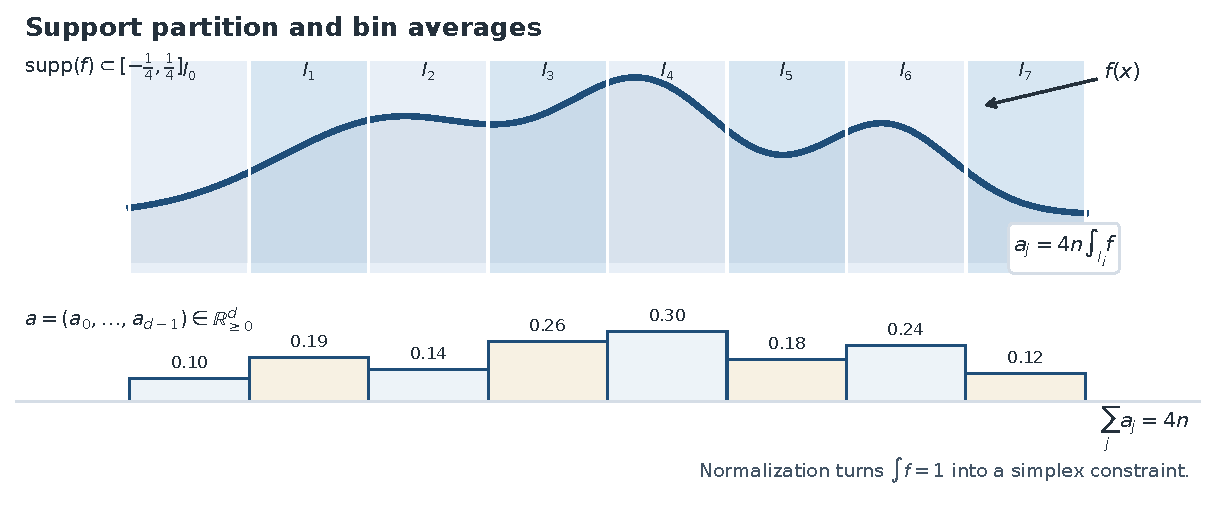
\includegraphics[width=\linewidth]{01_partition_bins.pdf}
\caption[A nonnegative profile on the support interval and its induced bin averages.]{A nonnegative profile supported on $[-\tfrac14,\tfrac14]$,
together with the half-open partition into equal bins.  The upper panel
shows the support decomposition, while the lower panel records the
induced averages $a_i=4n\,\mu_i$ and the simplex identity
$\sum_i a_i=4n$ after normalizing $\int f=1$.}
\label{fig:partition-bins}
\end{figure}

\subsection[Window Lower Bound for the Ratio]{Window Lower Bound for the Ratio}

The next lemma is the analytic bridge from the continuous problem to
the discrete windowed expressions of Cloninger and
Steinerberger~\cite[Lemma~1]{CS17}.

\begin{lemma}[Per-window test-value bound]
\label{lem:bin-reduction}
Let $f\in\mathcal{F}$ satisfy $\int f=1$, and let
$a_i=4n\int_{I_i}f$.  Then for every pair of integers
$\ell\ge 2$ and $s_{\mathrm{lo}}\ge 0$,
\[
  \|f*f\|_{L^\infty}
  \;\ge\;
  \frac{1}{4n\ell}
  \sum_{s=s_{\mathrm{lo}}}^{s_{\mathrm{lo}}+\ell-2}
  \ \sum_{\substack{0\le i,j\le d-1\\ i+j=s}}
  a_i a_j.
\]
\end{lemma}

\begin{proof}[Proof sketch]
Write $f_i=f\,\mathbf{1}_{I_i}$.  Then
$f=\sum_i f_i$ and $(f*f)(t)=\sum_{i,j}(f_i*f_j)(t)$.  The support of
$f_i*f_j$ is contained in $I_i+I_j$, an interval of length
$\tfrac{1}{2n}$ whose location depends only on $i+j$.  If one fixes
the sum-index window
$s_{\mathrm{lo}}\le i+j\le s_{\mathrm{lo}}+\ell-2$, the corresponding
Minkowski sums form an interval of total length $\tfrac{\ell}{4n}$.
The total $L^1$ mass contributed by these terms is
\[
  \sum_{s=s_{\mathrm{lo}}}^{s_{\mathrm{lo}}+\ell-2}
  \ \sum_{i+j=s}
  \frac{a_i}{4n}\frac{a_j}{4n}.
\]
Applying the averaging inequality
$\|h\|_{L^\infty}\ge |J|^{-1}\int_J h$ to this interval gives the
claimed lower bound.
\end{proof}

The Lean counterpart is
\texttt{continuous\_test\_value\_le\_ratio}, stated per window;
the maximized version follows by taking the supremum over all admissible
$(\ell,s_{\mathrm{lo}})$.

Geometrically, the products $a_i a_j$ quantify how much mass from
bins $i$ and $j$ can contribute to the autoconvolution.  Narrow windows
carry the favorable prefactor $\tfrac{1}{4n\ell}$ but capture fewer
pairs; wider windows capture more pairs but average over a longer
interval.  The branch-and-prune computation exploits this trade-off.


% ======================================================================
\section{Discretization of the Simplex}\label{sec:disc}
% ======================================================================

Having reduced the problem to minimizing over the continuous simplex
$A_n$, we face a new obstacle: $A_n$ is uncountable.  To bring the
problem within reach of a computer, we discretize the normalized mass
simplex $\Delta_n$.  Regular simplex grids are standard in
finite-dimensional optimization~\cite{Bomze2014}; here the key point is
that the formal proof uses a particular lattice point selected by a
cumulative-floor rule.

\subsection{The Lattice}

Fix a positive integer $m$.  In normalized mass coordinates, the
natural grid has spacing $1/m$.

\begin{definition}
Fix a positive integer $m$ (the ``grid resolution'').  The
\emph{discrete lattice} is
\[
  B_{n,m} \;=\; \left\{
    b \in \left(\tfrac{1}{m}\N\right)^d
    \;\middle|\;
    \sum_{j=0}^{d-1} b_j = 1
  \right\},
\]
where each $b_j$ is a nonnegative multiple of $\tfrac{1}{m}$.
\end{definition}

Equivalently, writing $c_i = m b_i$, the lattice consists of
nonnegative integer vectors $c = (c_0, \ldots, c_{d-1})$ with
$\sum c_j = m$.  These are the \emph{compositions} of the integer $m$
into $d$ nonnegative parts.

Figure~\ref{fig:simplex-lattice} shows this discretization on a
two-dimensional toy simplex, where a continuous point is rounded to a
nearby lattice point.

\begin{figure}[t]
\centering
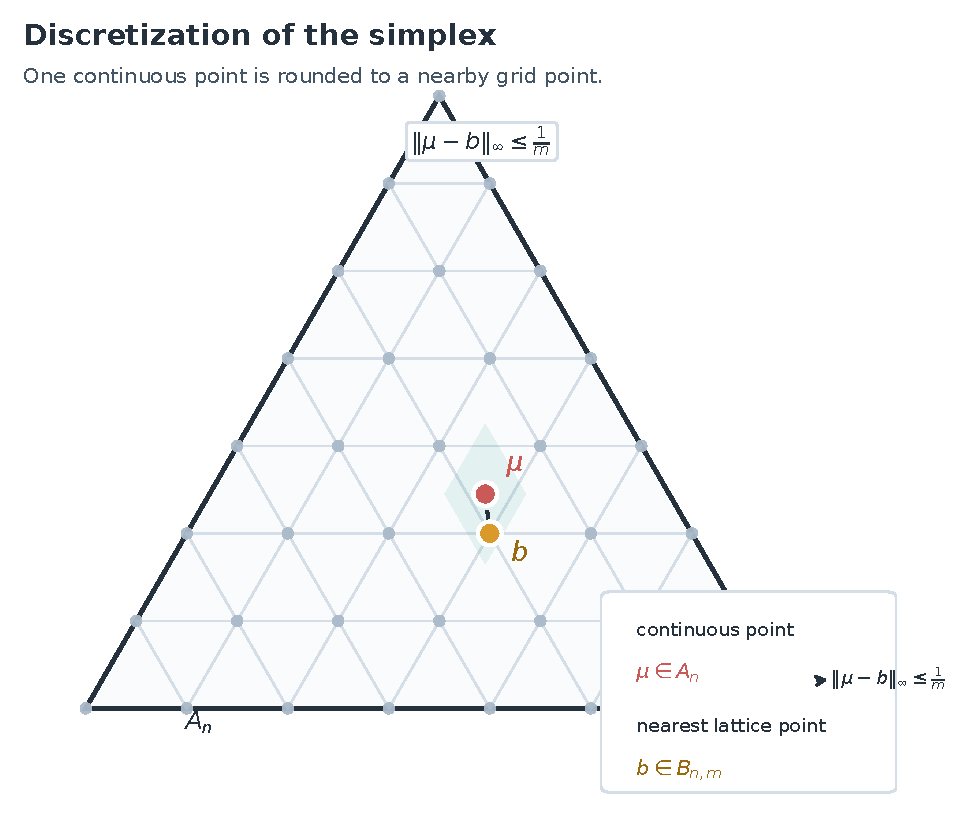
\includegraphics[width=0.76\linewidth]{02_simplex_lattice.pdf}
\caption[A three-coordinate slice of the normalized simplex and its lattice approximation.]{A three-coordinate slice of the normalized simplex.  The point
$\mu$ is replaced by a nearby lattice point $b \in B_{n,m}$; in the
formal proof this representative is chosen by the cumulative-floor map
described below.}
\label{fig:simplex-lattice}
\end{figure}

For the formal argument, however, one needs a specific lattice point,
not merely an existence statement.

\begin{definition}[Canonical discretization]
\label{def:canonical-disc}
Let $\mu\in\Delta_n$ and define the cumulative masses
\[
  M(k) \;=\; \sum_{i<k}\mu_i,
  \qquad 0\le k\le d.
\]
Set
\[
  D(k) \;=\; \lfloor m\,M(k)\rfloor,
  \qquad 0\le k\le d,
\]
and define the integer composition
$c=(c_0,\dots,c_{d-1})$ by
\[
  c_i = D(i+1)-D(i)\quad (0\le i\le d-2),
  \qquad
  c_{d-1}=m-D(d-1).
\]
The associated normalized lattice point is $w_i=c_i/m$.
\end{definition}

More precisely, the Lean definition
\texttt{canonical\_discretization} is applied to the function $f$ and
writes
\[
  D_f(k)
  \;=\;
  \left\lfloor
    m\,
    \frac{\sum_{i<k}\mu_i}{\sum_j \mu_j}
  \right\rfloor
\]
in terms of the bin masses $\mu_i=\int_{I_i}f$.  By
Lemma~\ref{lem:sum-bin-masses}, the denominator is~$1$ once
$\int f=1$, recovering Definition~\ref{def:canonical-disc}.

\begin{proposition}[Basic properties of the canonical discretization]
\label{prop:canonical-disc-basic}
The composition $c$ from Definition~\ref{def:canonical-disc} satisfies
\[
  \sum_{i=0}^{d-1} c_i = m,
  \qquad
  \left| \frac{c_i}{m} - \mu_i \right| \le \frac{1}{m}
  \quad\text{for each } i.
\]
\end{proposition}

\begin{proof}[Proof sketch]
The sum identity is telescoping:
\[
  \sum_{i=0}^{d-2} (D(i+1)-D(i)) + m-D(d-1) = m.
\]
For the coordinate error, write
\[
  \frac{c_i}{m}-\mu_i
  =
  \left(\frac{D(i+1)}{m}-M(i+1)\right)
  -
  \left(\frac{D(i)}{m}-M(i)\right),
\]
and use the elementary floor bounds
$-1<\lfloor x\rfloor-x\le 0$.  In Lean these statements are formalized
by \texttt{canonical\_discretization\_sum\_eq\_m} together with the
coordinatewise estimate proved in
\texttt{Sidon/DiscretizationError.lean}.
\end{proof}

\subsection{The Discretization Error Bound}

Define the set of \emph{contributing bins} for a window
$(\ell,s_{\mathrm{lo}})$ by
\[
  \mathcal{B}_{n,\ell,s_{\mathrm{lo}}}
  \;=\;
  \left\{
    i\in\{0,\dots,d-1\} :
    \exists\, j\in\{0,\dots,d-1\},\
    s_{\mathrm{lo}}\le i+j\le s_{\mathrm{lo}}+\ell-2
  \right\}.
\]
Equivalently,
\[
  \mathcal{B}_{n,\ell,s_{\mathrm{lo}}}
  =
  \left\{
    i :
    \max\!\bigl(0,s_{\mathrm{lo}}-(d-1)\bigr)
    \le i \le
    \min\!\bigl(d-1,s_{\mathrm{lo}}+\ell-2\bigr)
  \right\},
\]
which is the content of the Lean theorem
\texttt{contributing\_bins\_iff}.

The next estimate is the exact per-window bound used later in the main
theorem.

\begin{lemma}[Per-window discretization error]
\label{lem:disc-error}
Let $f\in\mathcal{F}$ satisfy $\int f=1$, let
$c$ be the canonical discretization from
Definition~\ref{def:canonical-disc}, and set
$w_i=c_i/m$.  For a fixed window $(\ell,s_{\mathrm{lo}})$, write
\[
  W \;=\; \sum_{i\in \mathcal{B}_{n,\ell,s_{\mathrm{lo}}}} w_i.
\]
Then
\[
  \operatorname{TV}_{n,m}(c;\ell,s_{\mathrm{lo}})
  -
  \operatorname{TV}^{\mathrm{cont}}_n(f;\ell,s_{\mathrm{lo}})
  \;\le\;
  \frac{4n}{\ell}
  \left(
    \frac{1}{m^2} + \frac{2W}{m}
  \right),
\]
where
\[
  \operatorname{TV}_{n,m}(c;\ell,s_{\mathrm{lo}})
  \;=\;
  \frac{1}{4n\ell}
  \sum_{s=s_{\mathrm{lo}}}^{s_{\mathrm{lo}}+\ell-2}
  \sum_{i+j=s}
  \left(\frac{4n}{m}c_i\right)\left(\frac{4n}{m}c_j\right),
\]
and $\operatorname{TV}^{\mathrm{cont}}_n(f;\ell,s_{\mathrm{lo}})$ is
the corresponding continuous expression from
Lemma~\ref{lem:bin-reduction}.
\end{lemma}

\begin{proof}[Proof sketch]
Write $w_i=\mu_i+\delta_i$.  Expanding the quadratic expression gives
linear and quadratic error terms.  The quadratic part is bounded by
$\tfrac{4n}{\ell}\cdot\tfrac{1}{m^2}$ because
$|\delta_i|\le \tfrac{1}{m}$, while the linear part is bounded by
$\tfrac{4n}{\ell}\cdot \tfrac{2W}{m}$ because only the contributing
bins matter in the chosen window.  This is precisely the estimate
proved in Lean before the theorem
\path{dynamic_threshold_sound}.
\end{proof}

\begin{corollary}[Global correction bound]
For every admissible window one has
\[
  \operatorname{TV}_{n,m}(c;\ell,s_{\mathrm{lo}})
  -
  \operatorname{TV}^{\mathrm{cont}}_n(f;\ell,s_{\mathrm{lo}})
  \;\le\;
  2n\left(\frac{2}{m}+\frac{1}{m^2}\right),
\]
because $W\le 1$ and $\ell\ge 2$.
\end{corollary}

\subsection{The Refined (Dynamic) Correction}

The global correction bound is convenient for estimates, but the formal
proof and the certificate computation use the sharper per-window
threshold.

\begin{theorem}[Dynamic threshold soundness]
\label{thm:dynamic-threshold}
Let $c$ be the canonical discretization of a normalized function
$f\in\mathcal{F}$ at parameters $(n,m)$, and let
\[
  W
  \;=\;
  \frac{1}{m}
  \sum_{i\in \mathcal{B}_{n,\ell,s_{\mathrm{lo}}}} c_i.
\]
If, for some window $(\ell,s_{\mathrm{lo}})$ with $\ell\ge 2$,
\[
  \operatorname{TV}_{n,m}(c;\ell,s_{\mathrm{lo}})
  \;>\;
  c_{\mathrm{target}}
  +
  \frac{4n}{\ell}
  \left(
    \frac{1}{m^2} + \frac{2W}{m}
  \right),
\]
then $R(f)\ge c_{\mathrm{target}}$.
\end{theorem}

\begin{proof}
Combine Lemma~\ref{lem:bin-reduction} with
Lemma~\ref{lem:disc-error}.  The first gives
$R(f)\ge \operatorname{TV}^{\mathrm{cont}}_n(f;\ell,s_{\mathrm{lo}})$,
and the second shows that the discrete test value exceeds the
continuous one by at most the correction term displayed above.
\end{proof}

The Lean counterpart is \texttt{dynamic\_threshold\_sound}.

\begin{remark}[Integer-coordinate form]
If
$W_{\mathrm{int}}=\sum_{i\in\mathcal{B}_{n,\ell,s_{\mathrm{lo}}}} c_i$,
then the threshold from
Theorem~\ref{thm:dynamic-threshold} can be written equivalently as
\[
  c_{\mathrm{target}}
  +
  \frac{4n}{\ell}\,
  \frac{1+2W_{\mathrm{int}}}{m^2}.
\]
This is the exact test-value threshold that reappears in the terminal
certificate at $(n,m)=(64,20)$.
\end{remark}

% ======================================================================
\section{The Windowed Test Value}\label{sec:testvalue}
% ======================================================================

With the discretization machinery in hand, we can describe precisely
what the algorithm computes at each lattice point.

\subsection{Definition}

\begin{definition}
For a mass vector $a = (a_0, \ldots, a_{d-1})$ with $a_i \ge 0$ and
$\sum a_i = 4n$, the \emph{autoconvolution} is the vector of length
$2d - 1$:
\[
  \conv[s] \;=\; \sum_{\substack{i + j = s \\[1pt] 0 \le i,j \le d-1}}
  a_i\, a_j,
  \qquad s = 0, 1, \ldots, 2(d-1).
\]
The \emph{test value} is
\[
  \tv(a) \;=\;
  \max_{\substack{2 \le \ell \le 2d \\[2pt] 0 \le k \le 2(d-1) - (\ell-2)}}
  \frac{1}{4n\ell}
  \sum_{s=k}^{k+\ell-2} \conv[s].
\]
\end{definition}

In words: compute the autoconvolution, slide a window of each possible
width $\ell$ across it, sum the $\ell - 1$ consecutive entries in each
window position, normalize by $4n\ell$, and take the maximum.

(The Lean definition \texttt{max\_test\_value} lets~$s_{\mathrm{lo}}$
range over all values $0,\dots,2d-1$; positions where the window extends
past the support of~$\conv$ contribute only zeros and do not change the
maximum.)

\begin{remark}[Integer composition coordinates]
The code stores compositions
$c=(c_0,\ldots,c_{d-1}) \in \N^d$ with $\sum_i c_i = m$ and recovers
the bin-average vector by
\[
  a_i \;=\; \frac{4n}{m}\,c_i.
\]
All pruning formulas below are stated in these integer
coordinates.
\end{remark}

\subsection{Efficient Computation via Prefix Sums}

The test value can be computed efficiently using prefix sums.  Let
$P[s] = \sum_{k=0}^{s} \conv[k]$ be the prefix sum of the
autoconvolution.  Then the windowed sum from $s_{\text{lo}}$ to
$s_{\text{hi}}$ is:
\[
  \sum_{s=s_\text{lo}}^{s_\text{hi}} \conv[s]
  \;=\;
  P[s_\text{hi}] - P[s_\text{lo} - 1]
  \qquad (\text{with } P[-1] = 0).
\]

The autoconvolution costs $O(d^2)$ per lattice point (an FFT-based
method would give $O(d \log d)$ but is slower in practice for the
moderate~$d$ values used here).  The prefix-sum construction and the
complete window scan each cost $O(d^2)$.

\subsection{Reversal Symmetry}\label{subsec:reversal}

A key structural observation cuts the search space in half.  If we
reverse the order of the bins, the autoconvolution peak does not change
--- intuitively, because convolution does not care which direction we
label the support.

\begin{theorem}[Autoconvolution Reversal Symmetry]
\label{thm:reversal}
For any mass vector $a$, $\tv(a) = \tv(\rev(a))$, where
$\rev(a) = (a_{d-1}, \ldots, a_0)$.
\end{theorem}

\begin{proof}
The argument has three moving parts.

\medskip
\noindent\textbf{Step 1: Autoconvolution reversal.}
Let $a' = \rev(a)$, so $a'_i = a_{d-1-i}$.  Then:
\[
  \conv'[s]
  \;=\; \sum_{i+j=s} a'_i a'_j
  \;=\; \sum_{i+j=s} a_{d-1-i}\, a_{d-1-j}.
\]
Substituting $i' = d-1-i$, $j' = d-1-j$ (so $i'+j' = 2(d-1) - s$):
\[
  \conv'[s] \;=\; \conv[2(d-1) - s].
\]
That is, the autoconvolution of the reversal is the reversal of the
autoconvolution.

\medskip
\noindent\textbf{Step 2: Window-sum bijection.}
A window sum of width $w = \ell - 1$ starting at $s_0$ transforms
under reversal to a window sum of the same width starting at
$2(d-1) - s_0 - w + 1$:
\begin{align*}
  \sum_{s=s_0}^{s_0+w-1} \conv'[s]
  &= \sum_{s=s_0}^{s_0+w-1} \conv[2(d-1)-s] \\
  &= \sum_{s'=2(d-1)-s_0-w+1}^{2(d-1)-s_0} \conv[s'].
\end{align*}
This is a window of the same width $w$, so the multiset of all window
sums at width $w$ is identical for $\conv$ and $\conv'$.

\medskip
\noindent\textbf{Step 3: Normalization preserves the maximum.}
The normalization $\tfrac{1}{4n\ell}$ depends only on $\ell$, not the
window position.  Since the multiset of window sums is identical at
each width, $\tv(a) = \tv(a')$.
\end{proof}

\begin{corollary}[Canonical Filter]
It suffices to check only \emph{canonical} integer compositions $c$
with $c \le \rev(c)$ lexicographically.  The associated bin-average
vectors have the same test value, so this halves the search space (up
to palindromes).
\end{corollary}

Figure~\ref{fig:reversal-canonical} depicts the reversal orbit of a
composition and the lexicographic canonicalization used to choose one
representative from each non-palindromic pair.

\begin{figure}[t]
\centering
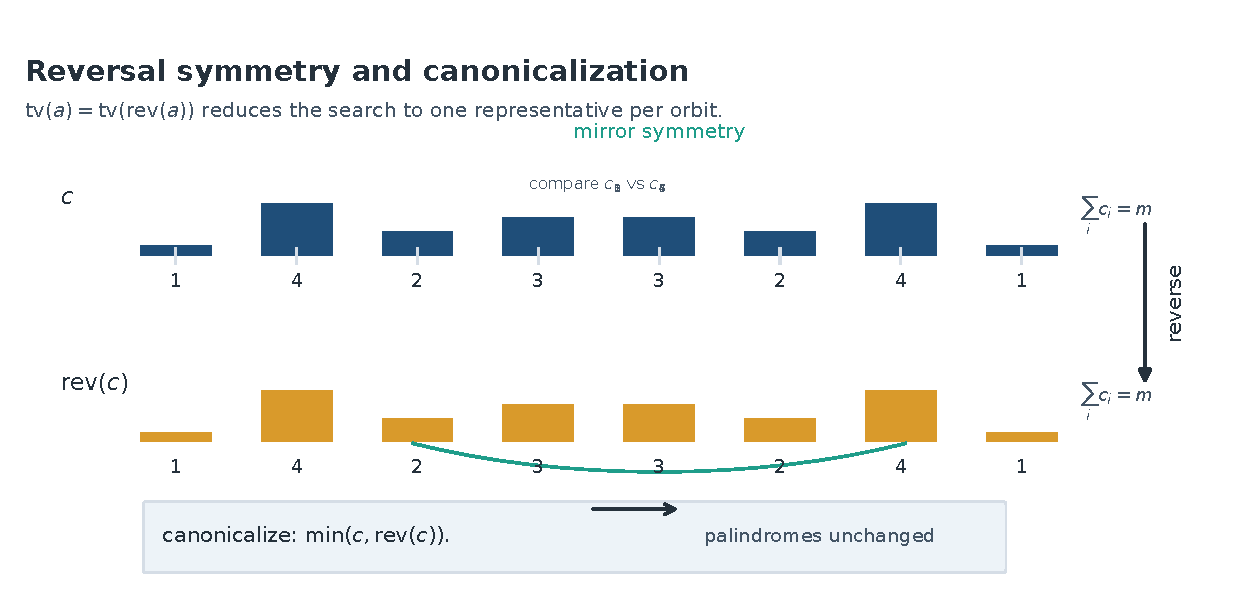
\includegraphics[width=0.92\linewidth]{03_reversal_canonical.pdf}
\caption[Reversal symmetry and canonicalization of compositions.]{Reversal symmetry of the test value and the canonicalization
rule $c \mapsto \min(c,\rev(c))$.  Palindromic compositions are fixed by
the involution, while non-palindromic pairs contribute only one
canonical representative to the search.}
\label{fig:reversal-canonical}
\end{figure}

Even after exploiting reversal symmetry, the number of integer
states to check --- roughly $\binom{m+d-1}{d-1}/2$ --- grows rapidly
with $d$ and $m$.  To keep the computation tractable, we need ways to
rule out large swathes of the simplex without computing the full test
value.


% ======================================================================
\section{Pruning Strategies}\label{sec:pruning}
% ======================================================================

\subsection{Asymmetry Pruning}

At first glance, the following bound might seem too crude to be useful:
it ignores everything about $f$ except how much mass sits on each half
of the support.  Yet in practice, this single test eliminates the vast
majority of configurations at every cascade level.

\begin{theorem}[Asymmetry Bound]
\label{thm:asymmetry}
Let $f \ge 0$ with $\supp(f) \subseteq (-\tfrac14, \tfrac14)$ and
$\int f = 1$.  Let $L = \int_{-1/4}^{0} f$ be the left-half mass.
Then:
\[
  \|f * f\|_{L^\infty} \;\ge\; 2L^2.
\]
\end{theorem}

\begin{proof}
Consider the left-left convolution:
\[
  (f * f)(t) \;=\; \int f(x)\, f(t-x)\, dx
  \;\ge\; \int_{-1/4}^{0} f(x)\, f(t-x)\, \mathbf{1}_{[-1/4,0]}(t-x)\, dx
\]
for $t \in (-\tfrac12, 0)$.  By Fubini's theorem, the total mass of
$f * f$ restricted to $(-\tfrac12, 0)$ is at least $L^2$ (the
left-left contribution).  Since $|(-\tfrac12, 0)| = \tfrac12$:
\[
  \|f * f\|_{L^\infty} \;\ge\; \frac{L^2}{1/2} \;=\; 2L^2.
\]
By symmetry, the same holds for the right-half mass $R = 1 - L$:
$\|f*f\|_\infty \ge 2R^2$.  Therefore
$\|f*f\|_\infty \ge 2 \max(L^2, R^2)$.
\end{proof}

\begin{corollary}[Asymmetry Threshold]
\label{cor:asym-threshold}
If $2L^2 \ge c_{\mathrm{target}}$, i.e.,
$L \ge \sqrt{c_{\mathrm{target}}/2}$, then the configuration is
ruled out.  The threshold left-mass fraction is:
\[
  p^* \;=\; \sqrt{c_{\mathrm{target}} / 2}.
\]
For $c_{\mathrm{target}} = 1.4$: $p^* \approx 0.8367$.
\end{corollary}

\begin{remark}[Exactness for step functions and under refinement]
For a step function already represented by a composition
$c = (c_0,\ldots,c_{d-1})$ with $\sum c_i = m$, the left-half mass is
\[
  L \;=\; \sum_{i < n} \frac{c_i}{m},
\]
because the midpoint $x = 0$ lies exactly on a bin boundary.  This
quantity is also preserved exactly under dyadic refinement: the left
child bins sum to the left parent bins.  Thus asymmetry pruning is an
exact statement for discrete step functions inside the cascade.
\end{remark}

\begin{remark}[Continuous-transfer caveat]
The asymmetry bound is a \emph{direct} $L^\infty$ bound on $f * f$.
It does \emph{not} go through the discretization framework of
Lemma~\ref{lem:disc-error}.  Accordingly, one must distinguish two
roles for asymmetry:
\begin{itemize}
  \item for an \emph{exact step function} represented by a composition
    $c$, the criterion is immediate and needs no correction term;
  \item inside the certificate computation, it serves as an
    inexpensive early pruning rule before the more expensive
    window scan.
\end{itemize}
The final Lean theorem no longer depends on carrying asymmetry
certificates through the continuous-to-discrete transfer.  Instead, the
formal theorem imports a stronger terminal-grid window certificate at
$d = 128$, so asymmetry remains part of the trusted external
computation but not part of the final analytic reduction.
\end{remark}

\begin{remark}[What the certificate computation prunes by]
The recorded cascade uses asymmetry pruning, the corrected
window-dependent threshold, reversal canonicalization, and the
single-bin cap from Section~\ref{subsec:energy-cap}.  The imported Lean
axiom does not encode these intermediate pruning mechanisms; it records
only the resulting terminal window witnesses.
\end{remark}

\subsection{Canonical Symmetry Exploitation}

If $c$ is an integer composition and
$\tilde c_i = \tfrac{4n}{m}c_i$ is its associated bin-average vector,
then Theorem~\ref{thm:reversal} gives
$\tv(\tilde c) = \tv(\widetilde{\rev(c)})$.  This motivates the
following notion of canonicality.

\begin{definition}
A composition $c$ is \emph{canonical} if $c \le \rev(c)$
lexicographically.  That is, comparing $c_0$ with $c_{d-1}$, then
$c_1$ with $c_{d-2}$, etc., $c$ comes first (or they are equal, i.e.,
$c$ is a palindrome).
\end{definition}

\begin{proposition}[Canonical Count]
\label{prop:canon-count}
For integer compositions of a fixed total mass $M$ into $d$ parts, the
number of canonical compositions is $\tfrac{N + P}{2}$, where
$N = \binom{M+d-1}{d-1}$ is the total count and $P$ is the number of
palindromes.
\end{proposition}

\begin{proof}
Every composition falls into exactly one of three categories:
palindromes (those equal to their own reversal), strictly canonical
non-palindromes ($b < \rev(b)$), and their reversals.  Since reversal
is an involution with no fixed points outside the palindromes, the
second and third categories have equal size $C$.  Counting gives
$N = P + 2C$, so the canonical count is $P + C = (N+P)/2$.
\end{proof}

\begin{remark}[Loop-bound tightening for $d = 4$]
For $b = (c_0, c_1, c_2, c_3)$ with total mass $M$ and
$c_3 = M - c_0 - c_1 - c_2$,
canonicality ($b \le \rev(b)$) requires $c_0 \le c_3$, giving three
loop bounds:
\begin{itemize}
  \item $c_0 \le \lfloor M/2 \rfloor$ \quad (if $c_0 > M/2$ then
    $c_3 < c_0$).
  \item $c_1 \le M - 2c_0$ \quad (need $c_2 \ge 0$ with
    $c_1 + c_2 \le M - 2c_0$).
  \item $c_2 \le M - 2c_0 - c_1$ \quad (ensures $c_3 \ge c_0$).
\end{itemize}
Plus a palindrome filter: when $c_0 = c_3$, require $c_1 \le c_2$.

For $d = 6$, analogous bounds apply: $c_0 \le \lfloor M/2 \rfloor$,
$c_4 \le M - c_0 - c_1 - c_2 - c_3 - c_0$, with equality checks for
the inner pairs when outer pairs tie.
\end{remark}


% ======================================================================
\section{The Multiscale Cascade}\label{sec:cascade}
% ======================================================================

Brute-force enumeration at fine resolution is hopelessly infeasible ---
even modest parameters yield billions of lattice points.  The key idea
is to start
coarse: most configurations can be ruled out cheaply at low resolution,
and only the stubborn survivors need to be examined more closely.

\subsection{Overview}

\begin{enumerate}[label=\textbf{Step \arabic*:}]
  \item \textbf{Start coarse.}  At level $L_0$, enumerate all
    canonical compositions of $m$ into $d_0 = 2n_0$ parts
    (e.g., $n_0 = 2$, $d_0 = 4$).

  \item \textbf{Prune.}  For each composition, apply asymmetry
    pruning and then scan windows using the corrected dynamic
    threshold.  If some window certifies the target bound, the
    composition is eliminated.

  \item \textbf{Refine survivors.}  Each surviving composition at
    resolution $d$ is refined to resolution $2d$ by \emph{dyadic
    splitting}: each bin is split into two sub-bins.

  \item \textbf{Repeat.}  Prune the refined compositions.  Continue
    until either all are eliminated (proof complete) or a
    computational budget is reached.
\end{enumerate}

Figure~\ref{fig:cascade-flow} summarizes the terminal certificate run,
including the exact survivor counts at each dyadic level.

\begin{figure}[t]
\centering
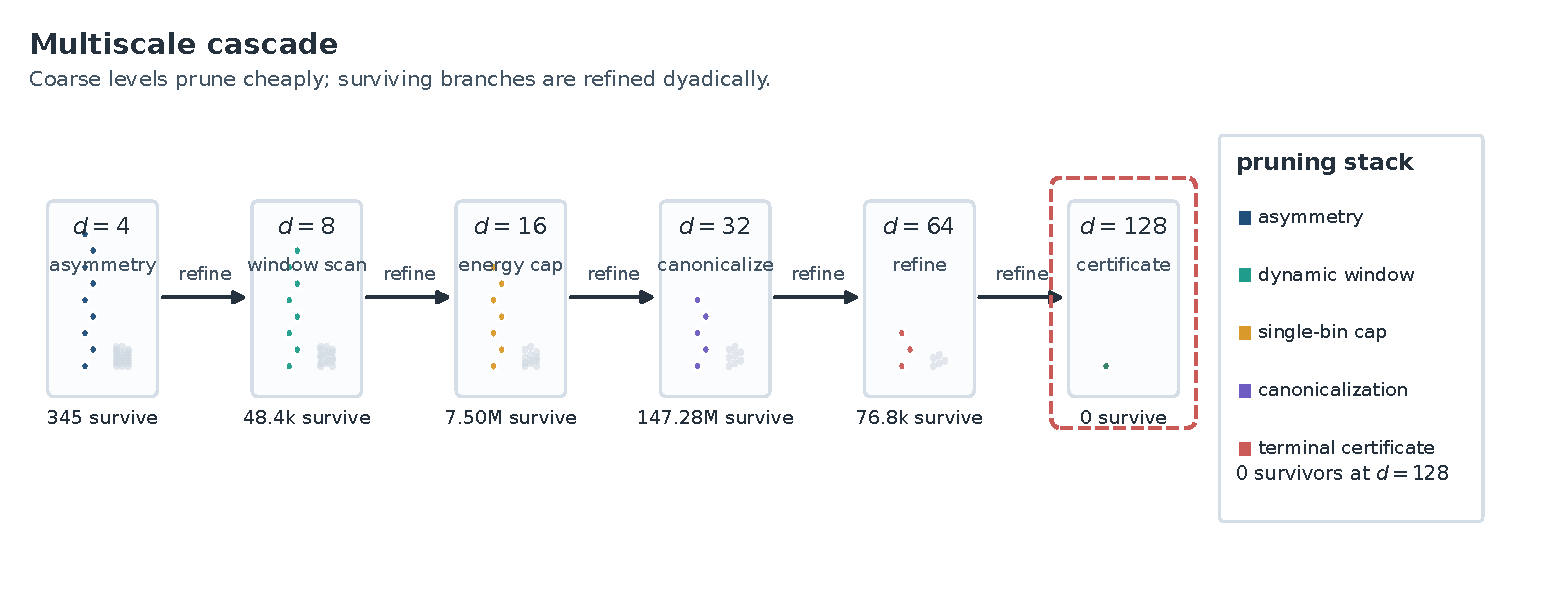
\includegraphics[width=\linewidth]{04_cascade_flow.pdf}
\caption[Stylized overview of the multiscale cascade with terminal-run survivor counts.]{Stylized overview of the multiscale cascade.  The annotations
record the exact survivor counts from the terminal certificate run: $345$ at
$d=4$, then $48{,}443$, $7{,}499{,}382$, $147{,}279{,}894$, $76{,}829$,
and finally $0$ at $d=128$.}
\label{fig:cascade-flow}
\end{figure}

\subsection{Dyadic Splitting (Refinement)}

Given a parent composition $b = (b_0, \ldots, b_{d-1})$ at resolution
$d$, the refinement produces children $c = (c_0, c_1, \ldots,
c_{2d-1})$ at resolution $2d$, where:
\[
  c_{2i} + c_{2i+1} \;=\; b_i \qquad \text{for each } i = 0, \ldots, d-1,
\]
with $c_{2i}, c_{2i+1} \ge 0$ and both being nonnegative integers.

\subsection{Energy Cap}\label{subsec:energy-cap}

One might worry that generating all possible children is wasteful.
Indeed, many children are immediately ruled out by the single-bin
diagonal window.  The energy cap avoids generating them in the first
place.

Recall that $a_j = \tfrac{4n_{\text{child}}}{m}c_j$ and the $\ell = 2$ diagonal window at
position $2j$ gives
\[
  \tv(a) \;\ge\; d_{\text{child}}\,\frac{c_j^2}{m^2},
  \qquad d_{\text{child}} = 2n_{\text{child}}.
\]
This yields the test-value cap
\[
  x_{\text{cap}}^{\mathrm{TV}}
  \;=\;
  \left\lfloor
    m \sqrt{\frac{c_{\mathrm{target}} +
      2n_{\text{child}}\left(\tfrac{2}{m} + \tfrac{1}{m^2}\right)
      + 10^{-9}}
    {d_{\text{child}}}}
  \right\rfloor.
\]
The implementation also applies the sharper direct cap
\[
  x_{\text{cap}}^{\mathrm{CS}}
  \;=\;
  \left\lfloor
    m \sqrt{\frac{c_{\mathrm{target}}}{d_{\text{child}}}}
  \right\rfloor,
\]
and uses
$x_{\text{cap}} = \min\!\left(x_{\text{cap}}^{\mathrm{TV}},
x_{\text{cap}}^{\mathrm{CS}}\right)$.

\begin{proposition}[Energy Cap Soundness]
If a child has some bin $c_j > x_{\mathrm{cap}}^{\mathrm{CS}}$, then
any nonnegative function with those child-bin masses already satisfies
$\|f*f\|_{L^\infty} > c_{\mathrm{target}}$.
\end{proposition}

\begin{proof}
Let $M_j = c_j/m$ be the mass in the $j$th child bin.  Restricting $f$
to that single bin produces a nonnegative function $f_j$ supported on
an interval of length $1/d_{\text{child}}$ and with total mass $M_j$.
By the same averaging argument used for asymmetry pruning,
\[
  \|f*f\|_{L^\infty}
  \;\ge\;
  \|f_j*f_j\|_{L^\infty}
  \;\ge\;
  \frac{M_j^2}{1/d_{\text{child}}}
  \;=\;
  d_{\text{child}}\,\frac{c_j^2}{m^2}.
\]
If
$c_j > m \sqrt{c_{\mathrm{target}}/d_{\text{child}}}$,
the right-hand side exceeds $c_{\mathrm{target}}$, which proves the
claim.
\end{proof}

\begin{remark}[Tighter Cauchy--Schwarz cap]
The looser cap $x_{\text{cap}}^{\mathrm{TV}}$ mirrors the older global
correction narrative, while the direct cap
$x_{\text{cap}}^{\mathrm{CS}}$ is the effective one in the
implementation.  It is tighter and does not need any discretization
correction term.
\end{remark}

\subsection{Terminal Certificate}

\begin{theorem}[Recorded Terminal-Grid Certificate]
\label{thm:cascade-sound}
For every composition $c = (c_0,\ldots,c_{127}) \in \N^{128}$ with
$\sum_{i=0}^{127} c_i = 20$, let
\[
  a_i \;=\; \frac{4 \cdot 64}{20}\, c_i,
  \qquad i = 0,\ldots,127,
\]
and let $\conv_a$ be the discrete autoconvolution of $a$.  Then there
exist integers $\ell \ge 2$ and
$s_{\mathrm{lo}}$ such that
\[
  \frac{1}{4 \cdot 64 \cdot \ell}
  \sum_{s=s_{\mathrm{lo}}}^{s_{\mathrm{lo}}+\ell-2} \conv_a[s]
  \;>\;
  \frac75
  +
  \frac{4 \cdot 64}{\ell}
  \left(
    \frac{1}{20^2}
    +
    \frac{2}{20^2}
    \sum_{i \in \mathcal{B}_{64,\ell,s_{\mathrm{lo}}}} c_i
  \right),
\]
where $\mathcal{B}_{64,\ell,s_{\mathrm{lo}}}$ is the set of contributing
bins for that window.
\end{theorem}

This is the computational claim imported into the Lean formalization as
the axiom \texttt{cascade\_all\_pruned}.  The dyadic cascade from $d=4$
to $d=128$ terminates with zero survivors at level~$L_5$; the
completeness properties in Section~\ref{sec:correctness} explain why
this terminal outcome implies the universal quantification above.  The
computation uses exact integer arithmetic for autoconvolutions and
conservative floating-point rounding for threshold comparisons; no
conclusion depends on floating-point correctness.

\subsection{Canonical Handling Across Levels}

At level $L_0$, only canonical compositions are generated.  At levels
$L_1$ and beyond, the situation is more subtle:

\begin{itemize}
  \item Children of a canonical parent $P$ are \emph{not} necessarily
    canonical.
  \item The reversal $\rev(P)$ is \emph{not} in the parent list
    (unless $P$ is a palindrome), so its children are not generated
    directly.
  \item However, if $C$ is a child of $P$, then $\rev(C)$ is a child
    of $\rev(P)$.  Since $\tv(C) = \tv(\rev(C))$
    (Theorem~\ref{thm:reversal}), testing $C$ suffices for both.
\end{itemize}

Therefore at levels $\ge 1$:
\begin{enumerate}
  \item Generate \emph{all} children of each parent (no canonical
    filter during generation).
  \item Test each child against the dynamic threshold.
  \item \emph{Canonicalize} survivors: replace each with
    $\min(C, \rev(C))$ lexicographically.
  \item \emph{Deduplicate}: remove duplicate canonical forms (children
    from different parents, or a palindrome parent producing both $C$
    and $\rev(C)$).
\end{enumerate}

\begin{proposition}[Completeness of Canonical Handling]
This procedure tests every composition at the child resolution:
if $C'$ is any child-level composition and $P' = \text{parent}(C')$,
then either $P'$ or $\rev(P')$ is in the parent list, and $C'$ or
$\rev(C')$ is among the tested children.
\end{proposition}

\subsection{Gray-Code Fused Kernel}

At deep cascade levels, each parent may have millions of children.
The current CPU kernel enumerates the same child set as the naive
Cartesian-product generator, but does so in mixed-radix Gray-code
order and fuses generation, pruning, canonicalization, and survivor
buffering into a single pass.  Consecutive children differ in exactly
one split coordinate, so the autoconvolution and tracked window mass
can be updated locally instead of recomputed from scratch:

\begin{itemize}
  \item \textbf{Incremental updates:} every Gray-code step changes one
    parent split, giving an $O(d)$ raw-convolution update and an
    $O(1)$ update of the tracked quick-check window mass.
  \item \textbf{Quick-check and ordered scans:} the previous killing
    window is retried first; if that fails, windows are scanned in a
    profile-guided order, but every admissible
    $(\ell,s_{\mathrm{lo}})$ is still checked before a child is
    declared a survivor.
  \item \textbf{Lookup-table thresholds and staged survivor writes:}
    the conservative integer threshold is precomputed as a table in
    $(\ell,W_{\mathrm{int}})$, and surviving rows are batched through
    an L1-resident staging buffer before they are flushed to the main
    output array.
  \item \textbf{Block skipping:} subtree pruning uses partial
    autoconvolutions of fixed prefixes, and the innermost Gray-code
    sweep can be fast-forwarded when a univariate range check proves
    that the same killing window eliminates the rest of that sweep.
\end{itemize}


% ======================================================================
\section{The Complete Proof}\label{sec:algorithm}
% ======================================================================

\subsection{Algorithm}

\begin{algorithm}[H]
\caption{Cascade Search For Terminal Coverage}
\label{alg:cascade}
\begin{algorithmic}[1]
\Require $c_{\text{target}}$, grid resolution $m$, starting half-bins
  $n_0$, max levels $L_{\max}$
\State $d_0 \gets 2 n_0$
\State Generate all canonical compositions of $m$ into $d_0$ parts
  \Comment{integer composition coordinates}
\State Apply asymmetry pruning (threshold
  $\sqrt{c_{\text{target}}/2}$)
\State For every remaining composition, scan all windows and prune if
  some window exceeds the dynamic threshold from
  Theorem~\ref{thm:dynamic-threshold}
\State $\text{survivors}_0 \gets$ unpruned compositions
\For{$k = 1, 2, \ldots, L_{\max}$}
  \State $d_k \gets 2 d_{k-1}$; \quad
    $n_k \gets 2 n_{k-1}$
  \State Compute the single-bin child cap
    $x_{\text{cap}} = \min(x_{\text{cap}}^{\mathrm{TV}},
    x_{\text{cap}}^{\mathrm{CS}})$
  \ForAll{parent $P \in \text{survivors}_{k-1}$}
    \ForAll{children $C$ of $P$ in mixed-radix Gray-code order (dyadic split with energy cap)}
      \State Apply asymmetry pruning to $C$
      \If{not asymmetry-pruned}
        \State Re-try the previous killing window; if needed, scan all windows of $C$ in profile-guided order using the lookup-table threshold
        \If{some window exceeds the dynamic threshold}
          \State Prune $C$
        \Else
          \State $C$ survives; canonicalize and store
        \EndIf
      \EndIf
    \EndFor
  \EndFor
  \State Deduplicate survivors (canonicalize $\to$ sort $\to$ scan)
  \State $\text{survivors}_k \gets$ deduplicated survivors
  \If{$|\text{survivors}_k| = 0$}
    \State \Return \textsc{Zero-Survivors}
  \EndIf
\EndFor
\State \Return \textsc{Inconclusive}:
  $|\text{survivors}_{L_{\max}}|$ compositions remain
\end{algorithmic}
\end{algorithm}

\subsection{Proof of the Main Theorem}

\begin{proof}[Proof of Theorem~\ref{thm:main}]
Normalize
\[
  g \;=\; \frac{f}{\int f},
\]
so that $\int g = 1$.  The autoconvolution ratio is scale-invariant,
so it suffices to prove $R(g)\ge \tfrac75$.

At parameters $(n,m)=(64,20)$, the identity
\texttt{sum\_bin\_masses\_eq\_one} gives total bin mass $1$, so the
cumulative-floor construction
\texttt{canonical\_discretization} produces a composition
$c\in\N^{128}$ with $\sum_i c_i=20$.  By the terminal certificate
Theorem~\ref{thm:cascade-sound}, there exist
$(\ell,s_{\mathrm{lo}})$ such that
\[
  \operatorname{TV}_{64,20}(c;\ell,s_{\mathrm{lo}})
  \;>\;
  \frac75
  +
  \frac{4\cdot 64}{\ell}
  \left(
    \frac{1}{20^2}
    +
    \frac{2}{20^2}
    \sum_{i\in\mathcal{B}_{64,\ell,s_{\mathrm{lo}}}} c_i
  \right).
\]
This is exactly the hypothesis of
Theorem~\ref{thm:dynamic-threshold}
(\texttt{dynamic\_threshold\_sound} in Lean), whose proof combines
the continuous lower bound
\texttt{continuous\_test\_value\_le\_ratio}
with the per-window discretization estimate from
Lemma~\ref{lem:disc-error}.  Therefore $R(g)\ge \tfrac75$, and
scale invariance gives $R(f)\ge \tfrac75$.

Taking the infimum over $f\in\mathcal{F}$ yields
$C_{1a}\ge \tfrac75$.
\end{proof}


% ======================================================================
\section{Soundness of the Computation}\label{sec:correctness}
% ======================================================================

The external computation matters only through the finite statement of
Theorem~\ref{thm:cascade-sound}.  To justify importing that statement,
one must verify that the implementation tested every relevant terminal
composition against the correct threshold.  We isolate five soundness
conditions and describe how each is verified.

\subsection{Complete Enumeration}

Every integer composition
$c \in \N^d$ with $\sum_i c_i = m$ must be either directly checked or
covered by a checked ancestor and all its refinements.
At $L_0$, the generator produces all $\binom{m + d_0 - 1}{d_0 - 1}$
compositions (verified against the stars-and-bars formula for all
parameter choices up to $d=16$, $m=20$), up to the reversal symmetry
from Section~\ref{subsec:reversal}; at $L_k$ ($k \ge 1$), all children
of all surviving parents are generated with no sampling.  Canonical
enumeration counts were checked against the exact count
$\tfrac{N+P}{2}$ from Proposition~\ref{prop:canon-count}.

\subsection{Window Exhaustion}

For each composition not eliminated by asymmetry, every valid
window $(\ell, k)$ with $2 \le \ell \le 2d$ and all valid starting
positions~$k$ is tested before the composition is declared a survivor.
An independent reference implementation agrees with the
optimized kernel on all $1{,}771$ canonical compositions at $(d,m)=(4,20)$.

\subsection{Conservative Arithmetic}

The autoconvolution is computed in exact integer arithmetic.  The
threshold comparison evaluates
\[
  c_{\text{target}}m^2\frac{\ell}{4n} + 1 + 2W_{\text{int}},
\]
with an added $10^{-9}m^2$ margin and a final
$(1 - 4\epsilon_{\text{mach}})$ factor before flooring.  The
multiplicative factor lowers the threshold, but the additive margin
dominates, so the net effect is conservative: the code may miss a
borderline prune but never falsely prunes.

\subsection{Refinement Completeness}

Every refinement of a surviving parent is checked at the finer level.
The dyadic splitting with energy cap generates all valid children
(Section~\ref{subsec:energy-cap}); children exceeding the cap are
provably pruned.  The Gray-code kernel produces identical canonical
survivor sets as the earlier lexicographic kernel on all tested parents.

\subsection{Terminal Cascade}

The cascade reached zero survivors at level~$L_5$
($d=4 \to 8 \to 16 \to 32 \to 64 \to 128$) after approximately
$70$ hours on a 128-core machine.  In the Lean formalization this
outcome is packaged as the axiom \texttt{cascade\_all\_pruned}: every
composition in~$\N^{128}$ of total mass~$20$ has some window whose test
value exceeds the corrected threshold at target~$\tfrac75$.

% ======================================================================
\section{Lean Formalization}\label{sec:formalization}
% ======================================================================

The accompanying formalization, carried out in
Lean~4~\cite{Lean4} on top of the Mathlib library~\cite{Mathlib},
consists of a modular development whose key analytic files are listed
in Table~\ref{tab:lean-map}.

Because \texttt{autoconvolution\_ratio} is encoded using
\texttt{ENNReal.toReal}, the formal theorem carries an explicit
finiteness hypothesis on the essential supremum of $f*f$.

The development is not axiom-free.  The analytic reduction is fully
proved in Lean; the single imported statement is the computational
certificate \texttt{cascade\_all\_pruned}, expressing the terminal-grid
statement at $d=128$.

\begin{table}[h]
\centering\small
\begin{tabular}{lll}
  \toprule
  \textbf{Paper statement} & \textbf{Lean name} & \textbf{File} \\
  \midrule
  Theorem~\ref{thm:main} & \texttt{autoconvolution\_ratio\_ge\_7\_5}
    & \texttt{FinalResult.lean} \\
  Theorem~\ref{thm:dynamic-threshold} & \texttt{dynamic\_threshold\_sound}
    & \texttt{DiscretizationError.lean} \\
  Lemma~\ref{lem:bin-reduction} & \texttt{continuous\_test\_value\_le\_ratio}
    & \texttt{TestValueBounds.lean} \\
  Lemma~\ref{lem:sum-bin-masses} & \texttt{sum\_bin\_masses\_eq\_one}
    & \texttt{TestValueBounds.lean} \\
  Lemma~\ref{lem:disc-error} & \texttt{discretization\_autoconv\_error}
    & \texttt{DiscretizationError.lean} \\
  Theorem~\ref{thm:cascade-sound} (axiom) & \texttt{cascade\_all\_pruned}
    & \texttt{FinalResult.lean} \\
  \bottomrule
\end{tabular}
\caption{Correspondence between paper statements and the Lean formalization.}
\label{tab:lean-map}
\end{table}


% ======================================================================
\section{Discussion}\label{sec:discussion}
% ======================================================================

\subsection{Relationship to the Original CS17 Proof}

Our framework is a direct extension of
Cloninger--Steinerberger~\cite{CS17}.  The key differences:

\begin{enumerate}
  \item \textbf{Dynamic correction}: We use a sharper per-window
    correction rather than only a coarse global bound.  This improves
    pruning while preserving rigor.

  \item \textbf{Multiscale cascade}: CS17 used $m = 50$ and refined
    from $n = 3$ through $n = 24$.  We use $m = 20$ with dyadic
    refinement from $d = 4$ through $d = 128$.

  \item \textbf{Fused generation}: Instead of materializing all
    children and then testing them, we generate and test each child
    inline, reducing memory from $O(N_{\text{children}} \cdot d)$ to
    $O(d)$ per parent.

  \item \textbf{Integer arithmetic}: Autoconvolution and threshold
    comparisons use exact integer operations, with floating-point
    involved only in the conservative threshold computation.
\end{enumerate}

\subsection{Limitations}

\begin{itemize}
  \item The proof is \emph{computer-assisted}: the mathematical
    argument reduces correctness to a finite computation, but that
    computation must be performed by a machine.  This paradigm is shared
    by other recent results where a finite but infeasible-by-hand
    verification completes a mathematical argument, notably the formal
    proof of the Kepler conjecture~\cite{Hales2017} and the numerical
    verification of the Riemann hypothesis up to
    $3\cdot 10^{12}$~\cite{PlattTrudgian2021}.

  \item The approach is limited by the exponential growth of the
    composition count with $d$ and $m$.  The multiscale cascade
    mitigates this, but very aggressive targets
    ($c_{\mathrm{target}}$ close to $C_{1a}$) will require more
    cascade levels and higher computational cost.

  \item The Lean theorem imports the terminal certificate
    \texttt{cascade\_all\_pruned} rather than replaying the full
    $70$-hour search inside the Lean kernel.  Eliminating this final
    axiom would require a kernel-level certification of the same finite
    computation.

  \item The formal statement isolates the case
    $\|f*f\|_{L^\infty} < \infty$ because of the way the ratio is
    encoded in Lean.  This is harmless for the lower bound on
    $C_{1a}$, since functions with unbounded self-convolution already
    satisfy every finite lower bound vacuously.
\end{itemize}


% ======================================================================
\section*{Acknowledgments}
% ======================================================================

This work builds on the foundational algorithm of Cloninger and
Steinerberger~\cite{CS17}.


% ======================================================================
% References
% ======================================================================

\bibliographystyle{amsalpha}
\bibliography{lower_bound_refs}

\end{document}
